\begin{figure}[h!]
    \centering
    
\includegraphics[width=0.8\textwidth]{pics/mongodb.png}
    \caption{MongoDB Logo}
    \cite{database_mongodb_logo}
    \label{fig:enter-label}
\end{figure}

\subsubsection{Grundlagen}
MongoDB ist eine dokumentenbasierte Datenbank, die für eine einfache Anwendungsentwicklung und Skalierung ausgelegt ist. Dabei gibt es drei verschiedene Möglichkeiten MongoDB zu verwenden: 
\begin{itemize}
    \item \textbf{MongoDB Atlas}
        \newline
        Dieses ist ein Multi-Cloud Datenbankdienst, welcher das Deployen und Verwalten der Datenbank vereinfacht, aber gleichzeitig die Vielseitigkeit bietet, die zum Erstellen von leistungsstarken Anwendungen benötigt werden.
    \item \textbf{MongoDB Enterprise}
        \newline
        Dies ist ein abonnementbasierte und selbstverwaltete Version von MongoDB und umfasst mehr Funktionen:
        \begin{itemize}
            \item \textbf{LDAP-Authentifizierung}
                \newline
                LDAP bedeutet "lightweight directory access protocol" und hilft Benutzern beim Finden von Daten über Organisationen und Personen. LDAP-Authentifikation verfolgt dabei folgende Ziele: Daten im LDAP Vezeichnis zu speichern und Benutzer beim Zugriff auf dieses Verzeichnis zu authentifizieren. Dabei ist LDAP eines der wichtigsten Authentifizierungsprotokolle, welches für Verzeichnisdienste entwickelt wurde.
                \cite{ldap_auth}
            \item \textbf{Kerberos Authentifizierung}
                \newline
                Ist ein Sicherheitsprotkoll, welches mit dem KDC (Key Distribution Center) arbeitet, welches alle Clients, User und Dienste verwenden müssen, um zu authentifizieren. Außerdem wird beim Authentifizierungsprozess ein KDC-Ticket vergeben. Dieses Authentifizierungsverfahren ist die Standardmethode für das Betriebssystem Microsoft Windows.
                \cite{kerberos_auth}
            \item \textbf{Audit Events}
                \newline
                Audit-Events sind sicherheitsrelevante Ereignisse in einem System zum Beispiel ein Verstoß gegen Systemzugriffskontroll- oder Verantwortlichkeitssicherheitsrichtlinien und melden diese Verstöße an den System-Audit-Logger, welcher als Teil des Kernels ausgeführt wird. Es werden Name des Ereignisses, Erfolg oder Misserfolg und alle anderen ereignisspezifischen Informationen übermittelt.
                \cite{audit_events}
\end{itemize}
    \item \textbf{MongoDB Community}
        \newline
        Dies ist der Source Code von MongoDB, welcher kostenlos und selbstverwaltet zur Verfügung steht.
\end{itemize}
\cite{mongodb_basics}

\subsubsection{Aufbau der Datenbank}
Die Datenbank ist in folgende Teile unterteilt:

\begin{itemize}
    \item \textbf{Fields}
        \newline
        Dies sind die kleinste Einheit in der Datenstruktur und würden in einer relationalen Datenbank einer Entität ensprechen.
    \item \textbf{Documents}
        \newline
        Documents entsprechen in einer relationalen Datenbank einem Datensatz und werden mittels BSON (Binary JSON) kodiert. Im Vergleich zu JSON ist es allein durch die visuelle Inspektion der beiden Formate nicht möglich, einen Unterschied festzustellen, da BSON auf dem JSON-Format aufbaut.
        \newline
        Der entscheidende Unterschied zwischen BSON und JSON liegt darin, dass BSON zusätzliche Datenformate wie Datumswerte und Binärdaten unterstützt. Dies wird durch kodierte Typ- und Längeninformationen ermöglicht, was wiederum zu einer erheblichen Leistungssteigerung beim Durchlaufen des Datensatzes führt. Die Integration von BSON ermöglicht es auch, Arrays und andere Dokumente effizient in diese Datensätze einzufügen.
        \newline
        Der Vorteil von "Documents" sind:
        \begin{itemize}
            \item Dokumente entsprechen in einigen Programmiersprachen nativen Datentypen
            \item Die Einbindung von Arrays und Documents vermeidet aufwendige JOINS
            \item Durch das dynamische Schema kann man die Datenbankstruktur sehr vielseitig gestalten
        \end{itemize}
        \begin{figure}[h!]
            \centering
            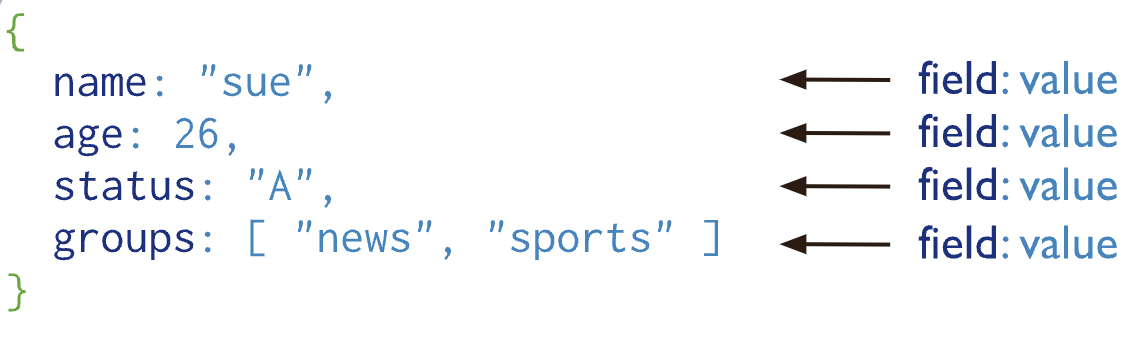
\includegraphics[width=0.8\textwidth]{pics/document.png}
            \caption{Document in MongoDB}
            \cite{mongodb_document}
            \label{fig:enter-label}
        \end{figure}
        \cite{mongodb_json_vs_bson}
    \item \textbf{Collections}
        \newline
        Die "Documents" werden in sogenannten "Collections" gespeichert, welche vergleichbar mit Tabellen in relationalen Datenbanken sind. Collections besitzen eine sogenannte "dynamic schema" Eigenschaft, was bedeutet, dass "Documents" in einer "Collection" unterschiedliche "Fields" besitzen können. Wie man im unten gezeigten Beispiel sieht, können beide dieser Documents in der selben Collection gespeichert werden.
        \begin{lstlisting}
            {"username": "admin", "firstname": "John"}
            {"lastname": "Doe"}
        \end{lstlisting}
        Man könnte also ausschließlich mit einer einzigen Collection arbeiten und in diese alle Datensätze speichern, man würde allerdings ziemlich schnell an seine Grenzen stoßen.
    \item \textbf{Cluster}
        \newline
        In einem Cluster sind alle Server der Datenbank gespeichert in denen sich die Collections befinden. Diese Cluster können Replica Sets sein, also Kopien aller Daten, oder Sharded-Cluster sein. Zu diesem Cluster wird im Laufe dieses Kapitels noch genauer eingegangen.
        \cite{mongodb_collections}
\end{itemize}

\subsubsection{Skalierung}
Die die Anzahl der Daten die gespeichert werden im Laufe der Zeit immer weiter anwächst, ist es wichtig seine Datenbank einfach skalieren zu können. 

\subsubsection{Horizontale Skalierung}
MongoDB wurde auf die horizontale Skalierung ausgelegt. Dazu müssen neue Maschinen (Server) dazugekauft werden, auf denen anschließend die Daten verteilt werden. Durch das dokumentenbasierte Datenmodell ist es wesentlich einfacher die Daten auf verschiedene Maschinen zu verteilen, dabei achtet MongoDB selbst darauf, dass alle Server annähernd gleich ausgelastet sind. Dazu werden Daten auch von einem Server auf einen anderen Server verschoben. Dazu verwendet MongoDB Shard-Schlüssel, welcher als Field in den Documents gespeichert wird und dient dazu die Documents in den Collections zu verteilen.
\cite{mongodb_collections}

Wie in der untenstehenden Grafik zu sehen, wird hier von "Shards" gesprochen. Das sogenannte Sharding stammt aus der Welt der traditionellen Datenbanken und beschreibt das zerteilen einer großen Datenbank in mehrere kleine. Die neu entstandenen kleinen Datenbanken nennt man Shards. Der Vorteil dieser Methode sind schnellere Schreib- und Lesezugriffe, da alle Shards in einem Cluster diese Befehle ausführen, wodurch ein hoher Grad der Parallelität erreicht wird.
\begin{figure}[h!]
    \centering
    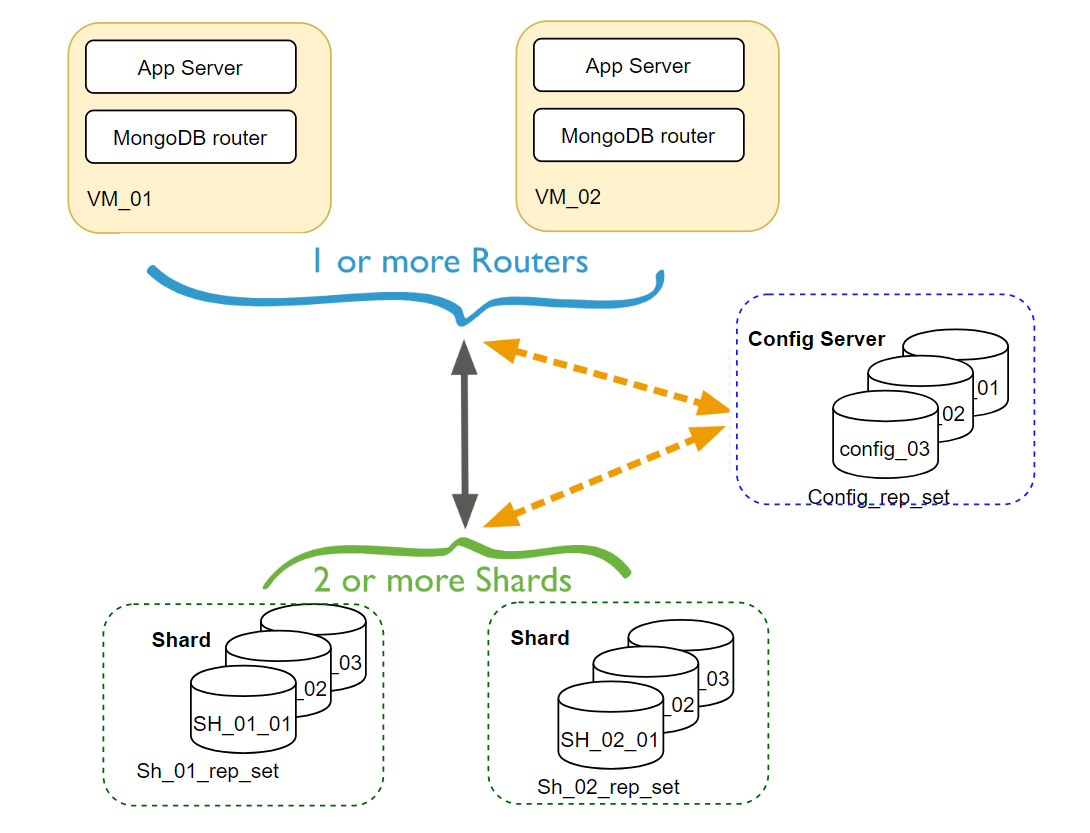
\includegraphics[width=0.6\textwidth]{pics/vertical_scaling_mongodb.png}
    \caption{Horizontale Skalierung MongoDB}
    \cite{vertical_scaling_mongodb}
    \label{fig:enter-label}
\end{figure}
\newline
MongoDB unterstützt zwei unterschiedliche Sharding-Methoden:
\begin{itemize}
    \item \textbf{Hashed Sharding}
        \newline
        Bei dieser Methode wird ein Hashwert aus dem Shard-Schlüssel gebildet und anschließend wird jedem Block ein Bereich zugewiesen, der auf den gehashten Wert basiert.
        \begin{figure}[h!]
            \centering
            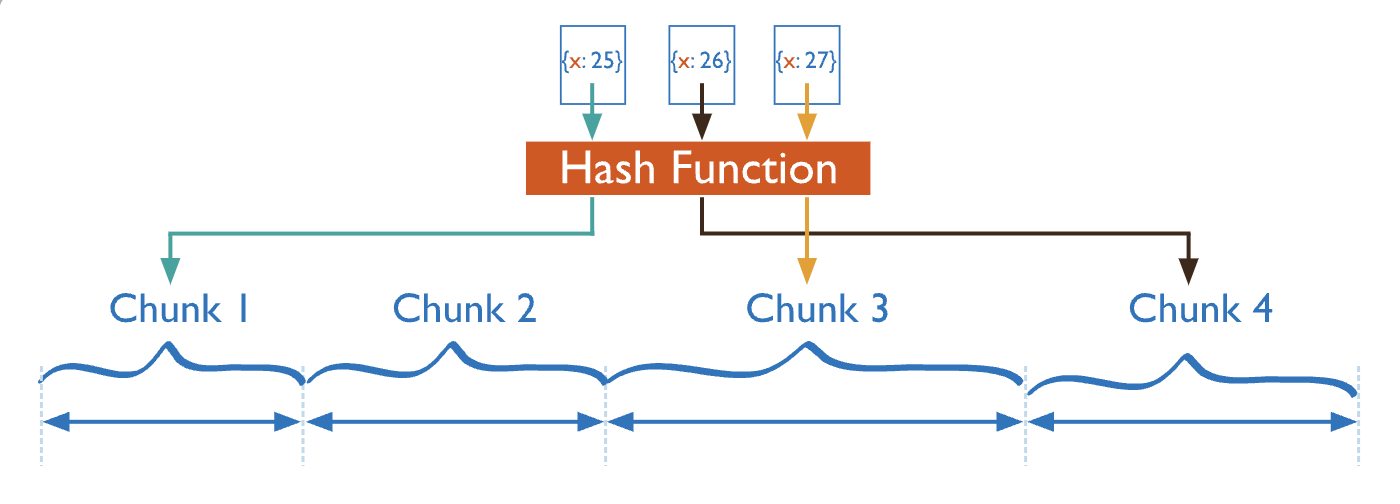
\includegraphics[width=0.5\textwidth]{pics/hashed_sharding.png}
            \caption{Hashed Sharding MongoDB}
            \cite{hashed_sharding_image}
            \label{fig:enter-label}
        \end{figure}
    \item \textbf{Ranged Sharding}
        \newline
        Bei dieser Methode werden die Daten aufgrund der Shard Schlüsselwerten in Bereiche unterteilt. Anschließend wird auf Basis der Shard-Schlüsselwerte  jedem Chunk ein entsprechender Bereich zugewiesen.
        \begin{figure}[h!]
            \centering
            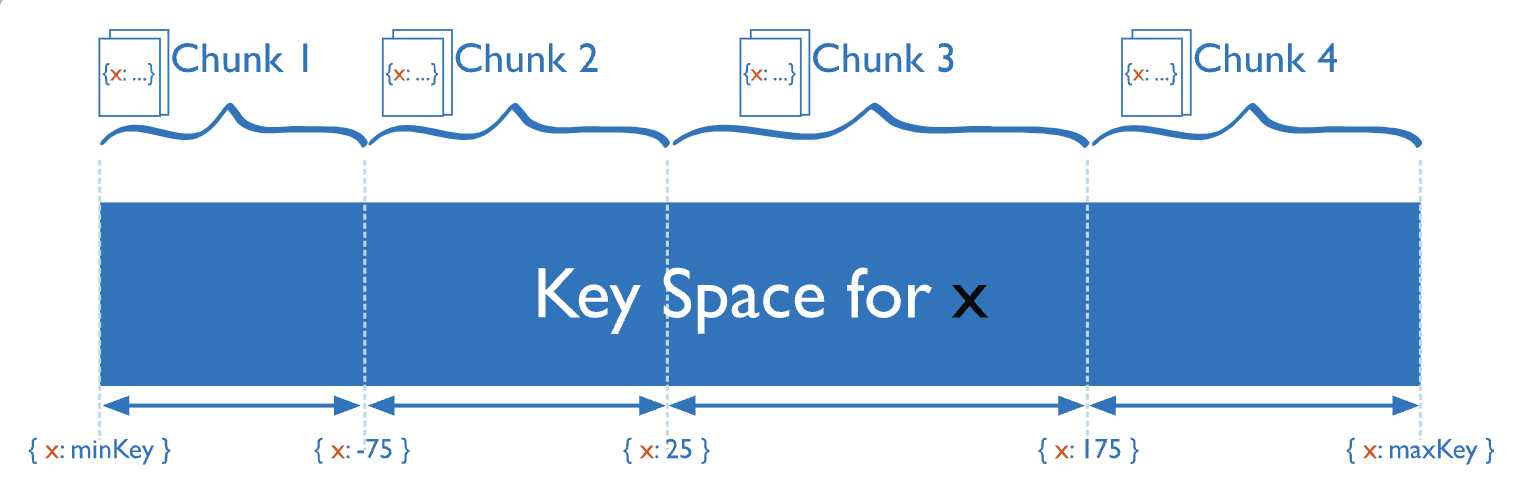
\includegraphics[width=0.5\textwidth]{pics/ranged_sharding.png}
            \caption{Ranged Sharding MongoDB}
            \cite{range_sharding_image}
            \label{fig:enter-label}
        \end{figure}
\end{itemize}

\subsubsection{Vertikale Skalierung}
Es gibt allerdings auch die Möglichkeit eine MongoDB Datenbank vertikal zu Skalieren. Dabei wird die Kapazität eines einzigen Servers gesteigert, indem man eine stärkere CPU, mehr RAM oder mehr Speicherplatz einbaut. In diesem Fall ist man allerdings an den technologischen Fortschritt angewiesen und es ist nicht unendlich möglich diese Skalierungsvariante zu verwenden. Des weiteren ist in den meisten Fällen eine horizontale Skalierung wesentlich kosteneffizienter als eine vertikale.
\cite{mongodb_sharding}

\subsubsection{Abfragen in MongoDB}
Dadurch, dass MongoDB keine relationale Datenbank ist, sehen die Abfragen auch anders aus wie bei SQL-basierte Datenbanken. In diesem Abschnitt wird auf die grundlegenden Abfragen in Kombination mit einem JavaScript Backend eingegangen. Bevor man allerdings mit den Abfragen beginnen kann, muss man zuerst eine Verbindung zur Datenbank aufbauen. Im untenstehenden Beispiel ist gezeigt wie dieser Verbinungsaufbau im Fall eines express.js Backends funktioniert.
\begin{lstlisting}
    const client = new MongoClient('<connection_string>')
    const result = client.connect()
    const db = result.db('<collection_name>')
\end{lstlisting}
Da nun die Verbindung zur Datenbank beseteht und eine Collection ausgewählt wurde (Zeile 3, obiger Codesnippet) kann man mit den Abfragen beginnen.
\newline
Möchte man aus einer Collection, Documents abfragen, gibt es zwei verschiedene Varianten, dies zu machen. Sind "einfache" Abfragen, wie zum Beispiel vergleiche von einzelnen oder mehreren Fields notwendig, benötigt es die "find"-Methode. In der "find"-Methode kann man die Query, in Form eines Objekts übergeben, lässt man es allerdings leer, werden alle Documents aus der Collection zurückgegeben.
\begin{lstlisting}
    const res1 = await db.collection.find({}).toArray()
    const res1 = await db.collection.find(
        {
            "firstname": "John"
        }
    ).toArray()
\end{lstlisting}
Wie im obigen Beispiel zu sehen ist, benötigt es nach der find-Methode eine weitere Methode, um das Ergebnis anzeigen zu können. Von diesen Methoden gibt es mehrere, anbei sind die zu finden, welche in dieser Diplomarbeit verwendet wurden.
\begin{center}
    \begin{tabular}{ | m{3cm} | m{2.3cm}| m{8cm} | } 
        \hline
        Name & Übergabetyp & Beschreibung \\ [0.5ex] 
        \hline\hline
        limit & number & Limitiert Documents die zurückgegeben werden \\
        \hline
        sort & object & Sortiert Documents nach Field z.B. \{'<field>': 1\} \\
        \hline
        project & object & Fields die zurückgegeben werden \\
        \hline
        skip & number & Überspringt n Documents \\
        \hline
    \end{tabular}
\end{center}
\cite{mongodb_query_methods}
Es können noch andere Methoden definiert werden, weitere Methoden sind im folgenden Link zu finden.
\newline
\url{https://mongodb.github.io/node-mongodb-native/3.6/api/Collection.html#find}
\newline
Um die Abfragen spezifischer zu gestalten, kann man auf verschiedene Operatoren zugreifen. Folgende Operatoren gibt es in MongoDB:
\begin{center}
    \begin{tabular}{ | m{1.5cm} | m{13cm} | } 
        \hline
        Name & Beschreibung \\ [0.5ex] 
        \hline\hline
        \$eq & Matches values that are equal to a specified value \\
        \hline
        \$gt & Matches values that are greater than a specified value \\
        \hline
        \$gte & Matches values that are greater than or equal to a specified value \\
        \hline
        \$in & Matches any of the values specified in an array \\
        \hline
        \$lt & Matches values that are less than a specified value \\
        \hline
        \$lte & Matches values that are less than or equal to a specified value \\
        \hline
        \$ne & Matches all values that are not equal to a specified value \\
        \hline
        \$nin & Matches none of the values specified in an array \\
        \hline
        \$and & Joins query clauses with a logical AND returns all documents that match the conditions of both clauses \\
        \hline
        \$not & Inverts the effect of a query expression and returns documents that do not match the query expression \\
        \hline
        \$nor & Joins query clauses with a logical NOR returns all documents that fail to match both clauses \\
    \end{tabular}
\end{center}
\begin{center}
    \begin{tabular}{ | m{1.5cm} | m{13cm} | } 
        \$or & Joins query clauses with a logical OR returns all documents that match the conditions of either clause \\
        \hline
        \$exists & Matches documents that have the specified field \\
        \hline
        \$type & Selects documents if a field is of the specified type \\
        \hline
        \$regex & Selects documents where values match a specified regular expression \\
        \hline
    \end{tabular}
\end{center}
\cite{mongodb_query_operations}
\newline
Die Syntax um oben dargestellten Befehle zu verwenden sieht wie folgt aus:
\newline
\begin{lstlisting}
    const res = await db.collection.find(
        {
            "firstname": { $exists: true }
        }
    ).toArray()

    const res1 = await db.collection.find(
        {
            $and: [
                "firstname": { $exists: true },
                "lastname": "Doe"
            ]
        }
    ).toArray()
\end{lstlisting}
\cite{mongodb_query_basics}
\newline
Möchte man nun allerdings nicht nur "einfache" Vergleichsabfragen durchführen, sondern möchte Documents gruppieren, oder einen Join auf eine andere Collection machen, benötigt man die Aggregation-Operation. Diese Operationen verarbeiten mehrere Documents, aus verschiedenen Collections, und können Berechnungen dieser Documents zurück geben. Es gibt zwei verschiedene Arten von Aggregation-Operationen:
\begin{itemize}
    \item \textbf{Aggregation Pipelines}
        \newline
         Eine Aggregation-Pipeline besteht aus einem oder mehreren Phasen, welche die Documents durchlaufen:
        \begin{itemize}
            \item In jeder Phase wird eine Operation an dem Document durchgeführt.
            \item Die Documents welche von einer Phase ausgegeben werden, werden an die nächste Phase übergeben.
            \item Gibt ein gruppiertes Ergebnis zurück, in dem man ein Minimum, Maximum, Durchschnitt oder Gesamtergebnis berechnen kann.
        \end{itemize}
        Im folgenden Beispiel wird eine Aggregation gezeigt, welche aus zwei Phasen besteht. Dabei filtert die ersten Phase die Bestellungen nach ihrer Größe und gibt alle Bestellungen an die nächste Phase weiter, welche die Größe Medium besitzen. In der zweiten Phase werden die übergeben Documents gruppiert und die Anzahl summiert.
        \begin{lstlisting}
            db.orders.aggregate( [
                // Phase 1
               {
                  $match: { size: "medium" }
               },
            
               // Phase 2
               {
                  $group: { _id: "$name", totalQuantity: { $sum: "$quantity" } }
               }
            ] )
        \end{lstlisting}
    \item \textbf{Single Purpose Aggregation Methods}
        \newline
        Diese Aggregation verarbeiten nur Documente aus einer einzigen Collection, sind daher auch nicht so mächtig wie die Aggregation-Pipelines. Es gibt folgende Aggregatinosmethoden:
        \begin{itemize}
            \item \textbf{estimatedDocumentCount()}
                \newline
                Diese Aggregation gibt die ungefähre Anzahl aller Documents in einer View oder Collection zurück.
            \item \textbf{count()}
                \newline
                Diese Aggregation gibt die genaue Anzahl aller Documents in einer View oder Collection zurück.
            \item \textbf{distinct()}
                \newline
                Gibt ein Array an Documents zurück, in dem nur Documents enthalten sind, welche in einem angegebenen Field nur unterschiedliche Werte besitzen.
        \end{itemize}
\end{itemize}
Im Zuge dieser Diplomarbeit war vor allem die Aggregation-Pipeline essentiell, des weiteren war auch die Single Purpose Aggregation Methode estimatedDocumentCount() für die Statistik-Seite  verwendet. Es wurde sich für diese Aggregation entschieden, da es nicht wichtig war, dass die Anzahl zu 100 Prozent korrekt ist und die Performance bei dieser Aggregation wesentlich besser ist.
\cite{mongodb_aggregation_basics}